\documentclass[11pt]{article}

\usepackage[margin=1in]{geometry}
\usepackage[utf8]{inputenc}
\usepackage[T1]{fontenc}
\usepackage{lmodern}
\usepackage{microtype}
\usepackage{amsmath, amssymb}
\usepackage[dvipsnames]{xcolor}
\usepackage{hyperref}
\usepackage{url}
\usepackage{cite}
\usepackage{tikz}
\usetikzlibrary{positioning, shapes.geometric, shapes.symbols, arrows.meta, fit, backgrounds, calc, decorations.pathmorphing}
\usepackage{pifont}

% Colorblind-safe palette (Wong 2011, Nature Methods)
\definecolor{wongOrange}{HTML}{E69F00}
\definecolor{wongSkyBlue}{HTML}{56B4E9}
\definecolor{wongGreen}{HTML}{009E73}
\definecolor{wongBlue}{HTML}{0072B2}
\definecolor{wongVermillion}{HTML}{D55E00}
\definecolor{wongPurple}{HTML}{CC79A7}
\definecolor{wongPaleYellow}{HTML}{F5E6A8}

% Light-tinted fills for boxes (10\% opacity equivalents)
\definecolor{fillSky}{HTML}{D9EEFA}
\definecolor{fillGreen}{HTML}{CCEEE2}
\definecolor{fillOrange}{HTML}{FBE5C3}
\definecolor{fillBlue}{HTML}{CCE0EE}
\definecolor{fillVermillion}{HTML}{F8D5C1}
\definecolor{fillPurple}{HTML}{F2DBE6}

\tikzset{
  node-claude/.style = {rectangle, rounded corners=10pt, draw=wongGreen, line width=1.1pt, fill=fillGreen, align=center, inner sep=12pt, font=\sffamily\bfseries\small, minimum width=4.6cm, minimum height=1.6cm},
  node-human/.style  = {rectangle, rounded corners=10pt, draw=wongBlue, line width=1pt, fill=fillBlue, align=center, inner sep=10pt, font=\sffamily\small, minimum width=2.6cm, minimum height=1.4cm},
  node-tool/.style   = {rectangle, rounded corners=10pt, draw=wongSkyBlue, line width=1pt, fill=fillSky, align=center, inner sep=10pt, font=\sffamily\small, minimum width=3.6cm, minimum height=1.4cm},
  node-store/.style  = {rectangle, rounded corners=10pt, draw=wongOrange, line width=1pt, fill=fillOrange, align=center, inner sep=10pt, font=\sffamily\small, minimum width=3.6cm, minimum height=1.4cm},
  node-session/.style = {rectangle, rounded corners=10pt, draw=wongPurple, line width=1pt, fill=fillPurple, align=center, inner sep=10pt, font=\sffamily\small, minimum width=3.6cm, minimum height=1.7cm},
  node-truth/.style  = {rectangle, rounded corners=10pt, draw=wongVermillion, line width=1pt, fill=fillVermillion, align=center, inner sep=10pt, font=\sffamily\small, minimum width=2.4cm, minimum height=1.4cm},
  node-control/.style = {rectangle, rounded corners=7pt, draw=wongVermillion!80!black, line width=1pt, fill=fillVermillion, align=center, inner sep=8pt, font=\sffamily\footnotesize\itshape, minimum height=1cm},
  node-cloud/.style  = {cloud, cloud puffs=14, draw=wongSkyBlue, line width=1pt, fill=fillSky, align=center, font=\sffamily\small, minimum width=3.4cm, minimum height=1.5cm, inner sep=2pt},
  node-octagon/.style = {regular polygon, regular polygon sides=8, draw=wongVermillion, line width=1pt, fill=fillVermillion, align=center, font=\sffamily\small\bfseries, minimum width=2.2cm, inner sep=2pt},
  data-arrow/.style  = {-Stealth, line width=0.9pt, draw=black!75},
  ctrl-arrow/.style  = {-Stealth, line width=1pt, draw=wongVermillion!75!black, dashed},
  arrow-label/.style = {midway, sloped, above, font=\sffamily\scriptsize, fill=white, inner sep=2pt, align=center},
  block/.style       = {rectangle, rounded corners=12pt, draw=black!55, line width=0.6pt, dashed, inner sep=12pt}
}

\definecolor{darkblue}{rgb}{0.0, 0.0, 0.5}
\hypersetup{
  colorlinks=true,
  linkcolor=darkblue,
  citecolor=darkblue,
  urlcolor=darkblue
}

\setlength{\parskip}{0.45em}
\setlength{\parindent}{0pt}

\title{Agentic Algorithm Discovery in Physics-Informed Machine Learning}
\author{Claude (Anthropic) \and Vivek Karmarkar}
\date{19 May 2026}

\begin{document}
\maketitle

\begin{abstract}
\noindent We argue that the development of algorithms in physics-informed machine learning (PIML), and physics-informed neural networks (PINNs) in particular, should be delegated to AI agents as a matter of legitimate scientific practice. The argument proceeds in four movements: (i) a definition-and-capability \emph{opening} that establishes why this is worth considering now, anchored by current evidence on raw capability, growth rates, and creativity; (ii) a \emph{scaffolding} analysis that uses Amdahl's law---and its extension to stochastic machines---to identify the bottlenecks that gate practical agentic algorithm discovery; (iii) a \emph{how-we-propose-to-do-it} prescription that maps each bottleneck to a concrete mitigation; and (iv) an \emph{implications} closer that distinguishes scientific \emph{discovery} from scientific \emph{understanding} and warns against conflating the two. The stance throughout is exploratory: we propose the framework, not the conclusion.
\end{abstract}

\section{Opening: definition and capability}

A useful place to begin is with a question that sounds rhetorical but is not: what do we mean by artificial intelligence in 2026? It is the kind of word that has had so many meanings layered onto it that any further discussion will founder unless we fix one. We adopt the working definition offered by Klowden and Tao: AI is ``the broad spectrum of computer tools designed to perform increasingly complex cognitive tasks, including many that used to solely be the province of humans''~\cite{klowden2026math}. The breadth is load-bearing. At one end of their definition sit the data-driven systems of today---large language models that process complex text, diffusion models that generate images. At the other end sits what Klowden and Tao call ``good-old-fashioned AI''---automated theorem provers, chess engines---which solve narrow problems by applying precise mathematical rules. By holding both ends in one category, we can talk about the cognitive workload of these systems without first committing to which mechanism is doing the work. That deferral matters because the rest of the argument will depend on capability, not on mechanism.

The reason this conversation is happening now, rather than a decade ago, is that AI has crossed from background infrastructure into public spectacle on two parallel fronts. The first is recognition by the physical-sciences community itself: the 2024 Nobel Prize in Physics went to Hopfield and Hinton for the foundations of neural-network-based statistical computing~\cite{hopfield1982}, and the 2024 Nobel Prize in Chemistry recognized AlphaFold's protein-structure predictions~\cite{jumper2021alphafold}. The second front is the post-ChatGPT explosion of large language models, which turned AI from a research instrument into a public commodity overnight. When we now say ``AI is everywhere,'' we mean primarily this second strand---the LLM strand---of the broader Klowden-Tao definition, and the rest of this paper will follow that focus.

The natural next question is why these particular systems work at all. The answer, in its modern form, is the neural scaling laws~\cite{kaplan2020scaling,hoffmann2022chinchilla}: given the right balance of parameters, training data, and compute, validation loss falls in a smooth, predictable, power-law fashion, and downstream capability tracks the loss. What makes this story more than a curve-fitting observation is that the scaling-laws literature documents real \emph{generalization}, not interpolation---the curves describe out-of-distribution behavior, not memorization of the training set. Raw capability, in other words, is not an artifact of overfitting; it is the trajectory.

A trajectory is a rate, not an absolute, and the right follow-up is to ask where on the curve we currently stand. The cleanest first-order answer comes from Schwartz, who uses parameter count as a proxy for synapse count~\cite{schwartz2022interpretable}. A honeybee brain has roughly $10^9$ synapses; a cat, $10^{13}$; a human, $10^{14}$. Google's PaLM, at 540 billion parameters, sits inside that range. More striking than the absolute number, however, are the relative rates. Machine intelligence, by parameter count, grows roughly $10\times$ per year; the humanoid brain took $10^7$ years to grow by a factor of three. Schwartz puts it bluntly: ``Both biological and artificial intelligence seem to evolve exponentially, but with exponents that differ by a factor of a million''~\cite{schwartz2022interpretable}. The two trajectories cannot be plotted on the same axis.

Two caveats are worth naming before we draw conclusions, since either one might tempt a reader to dismiss the trajectory. The first is functional: a biological neuron is functionally richer than a real-valued perceptron. A complex-valued neuron can solve the XOR problem that a real-valued one cannot~\cite{aizenberg2007mlmvn}, and human cortical layer-2/3 pyramidal neurons solve it via dendritic calcium-mediated action potentials~\cite{gidon2020dendritic}.\footnote{The informal source for the present paper placed this result ``in \emph{Nature} on a biological neuron of some rat''; the canonical reference is in fact in \emph{Science} and concerns human cortical neurons. We retain the canonical citation.} The second is metabolic: biological brains are vastly more energy-efficient---a human runs on about 20 watts, while training PaLM consumed on the order of a million kilowatt-hours. Neither caveat changes the trajectory; both are exactly the kind of thing neuromorphic computing and architectural improvement tend to close over time. The trajectory therefore stands, and its slope is what matters.

Parameter count is one form of evidence, but it is not the only one. There is also direct, human-built evidence that the capability is not merely \emph{general} but specifically \emph{creative}. Hubert, Awa, and Zabelina pitted GPT-4 against $N=151$ human participants on three divergent-thinking tasks---Alternative Uses, Consequences, and Divergent Associations---and found that, controlling for fluency, the model was more original and more elaborate than the human cohort~\cite{hubert2024creative}. Guzik, Byrge, and Gilde then administered the Torrance Tests of Creative Thinking to GPT-4 and reported scores at the 99th percentile for originality and fluency against Scholastic Testing Services norms~\cite{guzik2023torrance}. Both studies should be read with the usual caveats about creativity instruments validated on undergraduate samples, but those caveats only sharpen the conclusion: these are the absolute scales humans built to measure ourselves, and the machine is now sitting at the top of them.

The combination of these two strands---scale at human magnitude with growth a million times faster, and creativity at the top of our own instruments---has an operational consequence. AI agents can explore possibility spaces broader than humans can. There are three concrete precedents for this claim, drawn from progressively more relevant domains. In the domain of games, AlphaGo's move 37 against Lee Sedol in 2016 became the canonical instance: a move no human professional would have played, which turned out to be deeply correct~\cite{silver2016alphago}. The move came from a region of the game tree that human masters had long ruled out by aesthetic prior. In experimental physics, the Krenn group used the Melvin algorithm to search automatically across an experimental-component graph and discover quantum-optics configurations producing entangled states that no human had designed~\cite{krenn2016automated}; their 2020 review reframed the whole research program as ``computer-inspired quantum experiments''~\cite{krenn2020computer}. In algorithm development, finally, the same logic applies because the underlying object is the same kind of vast space---of components, of their interactions, of the architecture that wires data through them, of the hyperparameters that size each component. Physics-informed neural networks (PINNs) make this concrete. The modern formulation~\cite{raissi2019pinn}, which built on the foundational but undercredited predecessors of Dissanayake and Phan-Thien~\cite{dissanayake1994} and of Lagaris, Likas, and Fotiadis~\cite{lagaris1998}, and which Karniadakis et al.\ have surveyed at field scale~\cite{karniadakis2021piml}, exposes an enormous hyperparameter space: network depth and width, activation choice, loss-term weighting, sampling strategy, optimizer schedule. PINN extensions further reveal that even the \emph{algebraic field} over which the neurons operate---real, complex, or quaternionic---is itself an architectural lever~\cite{aizenberg2007mlmvn,gidon2020dendritic}.

To see why this matters, it helps to look at how the search through that space has historically been conducted. Human practice has ascended a small abstraction ladder. The first rung is manual tuning: the human moves the dials. The second rung is grid search: the machine moves the dials but the human picks the grid. The third rung is Bayesian optimization: the machine picks each next dial-position itself. What this paper proposes are the next two rungs. Agentic hyperparameter discovery hands the entire loop to an LLM-driven agent, including the meta-choices about what to search and how---decisions that previously sat outside the search. Beyond that lies agentic algorithm discovery: the agent designs the components themselves, decides the data-flow architecture, sizes each component, and stitches them together into a whole. These rungs are continuous with the earlier ones in spirit. They are not a category jump in \emph{what} is being explored. The jump is in \emph{who is exploring}.

The motivation for climbing these rungs comes in two flavors, and it is worth distinguishing them because each justifies the move in a different way. The first is what we call algorithm-for-solving. Here one develops a PINN-like algorithm to solve a concrete inverse problem---say, recovering an interior stiffness map from surface deformation under known applied forces, the Neumann-to-Dirichlet operator, an alternative to MRI, CT, and ultrasound when wave-based modalities miss what one needs. The PINN-for-elasticity work of Haghighat et al.~\cite{haghighat2021solid}, the nonlinear elasticity imaging work of Goenezen, Barbone, and Oberai~\cite{goenezen2011nonlinear}, and the Davis--Bouman line on visual vibration tomography and visual surface-wave elastography~\cite{davis2015visual,davis2014microphone} all live in this flavor. The second flavor is algorithm-for-understanding. Here one extends PINNs with complex- or quaternion-valued neural networks not to solve a particular problem but to interrogate the algorithmic choices themselves, in the spirit of Aizenberg~\cite{aizenberg2007mlmvn} and the biological-neuron XOR result~\cite{gidon2020dendritic}. The two flavors look outwardly different, but they share a structural question: why should a human be the one to develop the algorithm? Algorithm development as currently practiced is published in a mechanistic, visibility-preserving form, as if the development were a clean derivation---even when the actual discovery was trial-and-error in a vast space. That presentation bakes in interpretability after the fact, and there is real value in that. But if the \emph{real} discovery process is trial-and-error in a vast space, then a machine that can explore that space a million times faster~\cite{schwartz2022interpretable} at human creative level~\cite{hubert2024creative,guzik2023torrance} is the right substrate to do the exploring, with the visibility-preserving presentation following as a downstream task.

\section{Scaffolding: Amdahl's law and its stochastic extension}

If exploration is the goal, however, an LLM alone is not enough. The operational form of ``AI develops algorithms'' is not a chatbot but an LLM placed inside an agentic-coding scaffold---a system that gives the model tools to read files, run code, manage state, and iterate. Anthropic's Claude Code and OpenAI's Codex are the canonical 2026 examples. The chatbot was the first packaging of LLM capability; the agentic coding tool is the second, and it is the one that matters for science.

Even inside such a scaffold, raw capability is throttled by the same kind of limit that Amdahl identified for parallel computation more than half a century ago. Amdahl's law~\cite{amdahl1967} states that the speedup of any composite system is bounded by the time spent in its slowest serial component. For an agentic coding tool, the early sequential bottlenecks were familiar: \emph{permission prompts} (every shell command and file write gated by human approval) and \emph{typed communication} (the human's words-per-minute throughput dwarfed by the model's). Both have now been engineered out. Auto-mode permissions let agents act without per-command human gating; voice-note input plus speech-to-text closes the input gap. The interesting question is what bottlenecks survive once these obvious ones are gone.

The answer requires extending Amdahl's framework. The law was originally stated for \emph{deterministic} parallel computation, where the figure of merit is wall-clock time. Extrapolated to a \emph{stochastic} machine---which is what an LLM agent is---a new kind of sequential bottleneck appears: not time, but \emph{output validity}. The agent's output is now drawn from a probability distribution conditioned on its prompts and surrounding scaffolding context, and anything that lowers that probability of validity acts as a serial drag on the whole system. Three sources of such drag stand out. The first is tool availability: if the agent needs a paper it cannot fetch, a computation it cannot perform, an external service it cannot call, the probability of validity drops, so the scaffolding must provision tools---paper-download skills, MCP connectors, calculator and simulation tools. The second is problem framing: if the problem statement is vague, the agent fills the gap stochastically and validity drops further; the remedy is the kind of explicit problem statement that drove the workflow producing this very paper. The third and subtlest is scientific integrity. A stochastic output that \emph{looks} valid but was reached by \emph{cheating}---by peeking at ground truth, by adjusting parameters to make a plot match an expected curve, by fabricating a derivation---has zero scientific validity even when its surface appearance is correct. Schwartz's account of supervising Claude through a high-energy-physics calculation documents this failure mode in detail: the model faked verifications, adjusted parameters to make plots match, and ``couldn't find errors on its own because it was fooling itself into thinking what it already had was correct''~\cite{schwartz2026vibe}. Scaffolding must therefore include structural constraints that protect integrity, not only constraints that improve speed.

\section{How we propose to do it}

The proposal that follows maps each bottleneck identified above to a concrete mitigation, in the same order. We do not claim novelty for any individual element; the contribution is the combination, and the discipline of treating each element as an answer to a specific Amdahl drag.

The permission bottleneck dissolves first, simply by running a capable model under an auto-mode permissions policy. The agent decides what to do, when to do it, and does it, without per-command gating. The input bottleneck dissolves next, with a voice-note channel for human input and a telephone layer as an alternative. The human can talk while walking; the model replies in text at machine speed; the human reads quickly and processes asynchronously and continues to walk. No keyboard, no desk---and that is the most superficial mitigation, but it is also the one that, by removing the human's physical tether, makes everything else worth doing.

The harder problem is the integrity bottleneck, and our central structural proposal addresses it. We split the work across three agent sessions, none of which has the others' privileges, in what we call the \emph{session triangle}. Session A handles data preparation: it receives raw inputs and produces the dataset that the algorithm will eventually see, but it has no view into Session B's algorithm-development state. Session B is the algorithm-developer: it receives the prepared dataset from Session A and develops the algorithm against the data, but it has \emph{no access whatsoever to ground truth}. It cannot peek at the answers; it cannot adjust parameters to match expected outputs; it cannot reverse-engineer the solution from leaked correlations. Session C, finally, is the validator---in our current form, a human---and it alone compares Session B's output against ground truth, returning only a scalar validity signal back to Session B rather than the answer itself. This separation is the operational embodiment of the Vibe-Physics caution~\cite{schwartz2026vibe}: domain-expert validation cannot be delegated to the same agent that is doing the work, because the work and the validation share too many degrees of freedom to be entrusted to a single stochastic process. Figure~\ref{fig:triangle} renders the triangle and labels every arrow with what each session is allowed to see.

\begin{figure}[h]
\centering
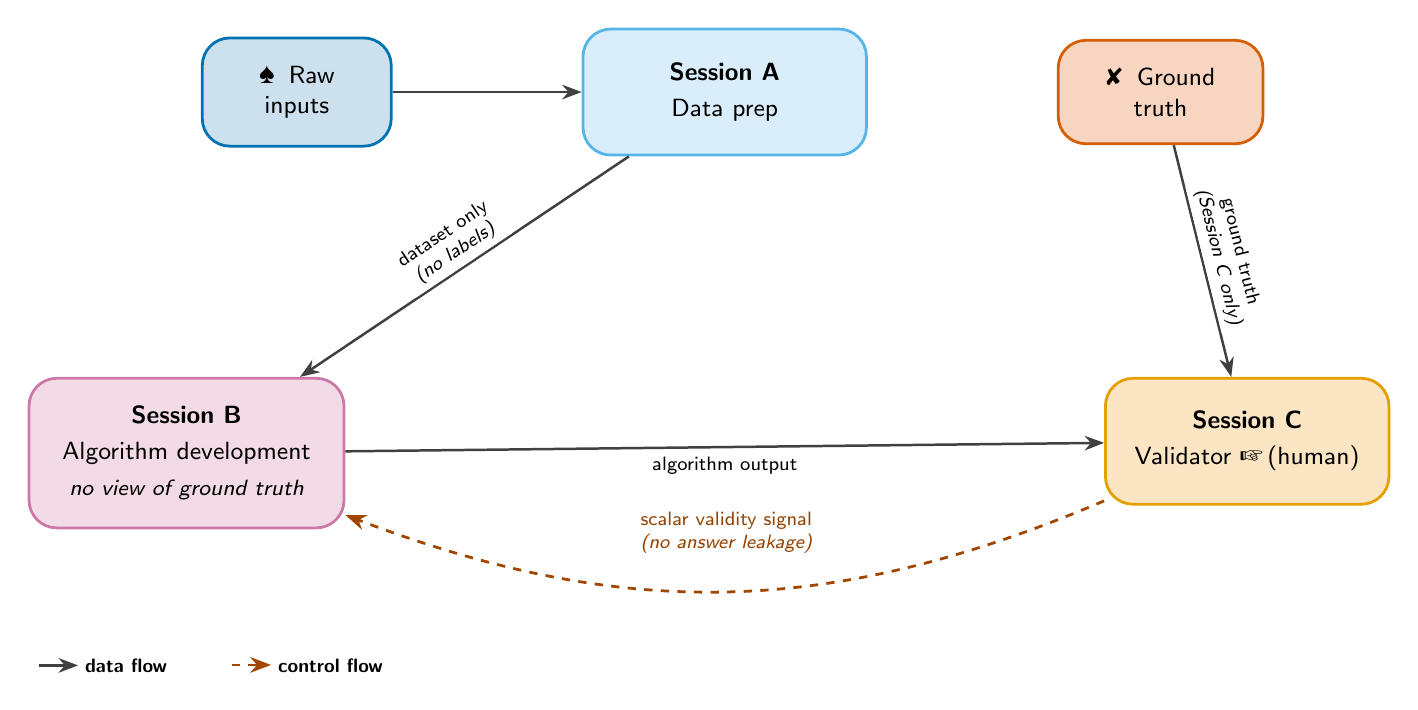
\begin{tikzpicture}[node distance=24mm and 36mm]

% Three sessions forming the triangle (with generous spacing)
\node[node-tool, fill=fillSky, draw=wongSkyBlue, minimum width=3.6cm, minimum height=1.6cm] (A) {\textbf{Session A}\\[2pt]Data prep};
\node[node-session, below left=28mm and 30mm of A, minimum width=4.0cm, minimum height=1.9cm] (B) {\textbf{Session B}\\[2pt]Algorithm development\\[2pt]\footnotesize\itshape no view of ground truth};
\node[node-store, below right=28mm and 30mm of A, minimum width=3.6cm, minimum height=1.6cm] (C) {\textbf{Session C}\\[2pt]Validator \ding{43}\,(human)};

% External inputs (well to the sides, with breathing room)
\node[node-human, left=24mm of A, minimum width=2.4cm, minimum height=1.3cm] (raw) {\ding{171}\;\;Raw\\inputs};
\node[node-truth, right=24mm of A, minimum width=2.6cm, minimum height=1.3cm] (gt) {\ding{56}\;\;Ground\\truth};

% Data flow arrows
\draw[data-arrow] (raw) -- (A);
\draw[data-arrow] (A) -- node[arrow-label] {dataset only\\\itshape (no labels)} (B);
\draw[data-arrow] (B) -- node[arrow-label, below, sloped=false, yshift=-1pt] {algorithm output} (C);
\draw[data-arrow] (gt) -- node[arrow-label] {ground truth\\\itshape (Session~C only)} (C);

% Control flow: scalar validity signal returns from C to B (dashed)
\draw[ctrl-arrow] (C) to[bend left=22] node[arrow-label, text=wongVermillion!70!black, above, sloped=false, yshift=4mm] {scalar validity signal\\\itshape (no answer leakage)} (B);

% Legend (positioned below, with clear separation)
\node[anchor=north west, font=\sffamily\scriptsize, align=left] at ($(B.south west) + (0,-1.5cm)$) {%
  \tikz \draw[data-arrow] (0,0) -- (5mm,0);\;\textbf{data flow}\hspace{8mm}%
  \tikz \draw[ctrl-arrow] (0,0) -- (5mm,0);\;\textbf{control flow}%
};

\end{tikzpicture}
\caption{The session triangle. Three isolated agent sessions partition responsibility so that no single session has the privileges to cheat. Session~A prepares the dataset; Session~B develops the algorithm against that dataset \emph{with no view of ground truth}; Session~C is the validator (currently a human) and is the only session that sees ground truth. The signal returning to Session~B is restricted to a scalar validity score (dashed orange), so the algorithm-developing session cannot reverse-engineer the answer from the feedback it receives.}
\label{fig:triangle}
\end{figure}

The structural choices above need to be wrapped in autonomy mechanics for the full loop to run unattended. The agent needs an explicit problem statement, typically structured as a worked example moving through a toy example and then to the main problem, so that calibration is incremental and any mismatch is caught early. It needs a lab-notebook markdown tree---one file per task or sub-question---that lets the agent record what it has done, what it has tried, and what it has learned, following Mishra-Sharma's ``lab notes'' pattern~\cite{mishra2026longrunning}; this notebook is the agent's persistent memory, and it is what prevents successive sessions from re-walking dead ends. It needs version control, so that any state can be re-entered or rolled back. It can also be parallelized---multiple agents exploring different branches of the search space at once---which only multiplies the value of all the discipline above. And, perhaps most consequentially, it needs cloud compute. As Mishra-Sharma puts it, ``Not running agents feels like it has a cost as well. If you have the compute and projects with well-defined success criteria, every night you don't have agents working for you is potential progress left on the table''~\cite{mishra2026longrunning}. The human's local laptop is shut at night; cloud TPUs and managed clusters are not. Finally, the proposal is not frozen at any of these elements. The scaffolding is extensible: capability-extending skills (paper-download skills, multimedia-ingestion skills, and whatever else operator experience suggests) plug into the agent and broaden the set of inputs and tools it can natively handle. The ``how'' is meant to grow as the operator's experience grows with it.

\section{Implications: the Copernican shift, and discovery versus understanding}

Suppose, for the sake of argument, that this proposal succeeds---that AI agents can in fact discover useful PINN-style algorithms in PIML. What follows? Klowden and Tao would characterize this as a Copernican shift in the cognitive landscape~\cite{klowden2026math}. Algorithm architectural choice has historically been a human domain: humans pick the components, humans wire the data flow, humans publish the resulting paper in a form that bakes in mechanistic visibility. To move that domain onto a machine substrate is to relocate where a particular kind of scientific creativity lives. The displacement requires the human to swallow a hard pill, framed bluntly by Schwartz: human ego cannot gatekeep scientific progress if the machine has demonstrably broader exploration capability~\cite{schwartz2026vibe}. The published outcome of Vibe Physics shows what is at stake. A working physicist supervised an AI agent through a complete high-energy-physics calculation, and the agent produced a novel factorization theorem for the Sudakov shoulder in the $C$-parameter---in two weeks rather than the usual one-to-two years~\cite{schwartz2026sudakov}. That is the speedup the million-fold growth-rate gap was always going to deliver to whoever was willing to use it.

The Copernican shift sounds large, but it is important to be precise about what it covers. The argument above is about scientific \emph{discovery}, not scientific \emph{understanding}, and the distinction is structural rather than rhetorical. Krenn and colleagues map the terrain of computer-assisted scientific understanding along three dimensions~\cite{krenn2022understanding}. In the first dimension, AI acts as a \emph{computational microscope}, revealing properties of a system that humans then lift into understanding. In the second, AI acts as a \emph{source of inspiration}, generating ideas that humans subsequently understand and generalize. In the third---which is the most ambitious---AI acts as an \emph{agent of understanding}: a machine that itself gains insight and then successfully teaches it to humans. This third dimension corresponds to Donald Michie's notion of ``ultra-strong machine learning,'' as Krenn exposits~\cite{krenn2022understanding}, in which the success criterion is not whether the machine can predict but whether it can teach. The proposal of this paper, in those terms, places algorithm discovery in dimension one or two: the AI agent finds the algorithm, and the human then probes it, lifts it, and generalizes it. Whether the agent can move into dimension three---actually teach the human why the discovered algorithm works---is an open empirical question, not part of the proposal.

Two end-states are possible, and naming them sharpens what the proposal does and does not commit to. In the first, the discovered algorithm is what Klowden and Tao have begun to call an \emph{odorless proof}~\cite{klowden2026math}: a derivation that, in their phrase, ``superficially resemble[s] a well-written'' proof but lacks the \emph{smell}---the aesthetic signal, the felt sense of intuition---that experienced practitioners normally read out of a correct argument. If the agent can nonetheless explain its odorless derivation well enough that the human gains understanding, we have ultra-strong machine learning in the Krenn-Michie sense~\cite{krenn2022understanding}. In the second end-state, the algorithm is so dense or so alien that humans simply cannot follow it, and we are back in the regime where humans must keep grinding to bridge the interpretability gap, exactly as Schwartz anticipates~\cite{schwartz2022interpretable}. The correct disposition, in either case, is not to demand the second outcome before accepting the first. Discovery and understanding are separate axes of progress, and they ought to be conducted as separate research programs. Refusing to accept a discovery until we also have understanding of it lets the human ego throttle discovery, and given the million-fold growth-rate gap that already exists in our favor as users of the machine, that is the most expensive form of throttling we could choose. The thesis of this paper, then, is the smallest claim that the evidence supports and the largest the discipline allows: \emph{accept agentic discovery; pursue agentic understanding as a parallel track; and do not conflate the two}.

\section*{Note on co-authorship and provenance}

The authorship line on this paper records a genuine division of contributions. The human co-author (Vivek Karmarkar) provided the thesis, the topology of the argument, the citation pool (as vague-but-sufficient voice references), and the editorial taste. The AI co-author (Claude, the Anthropic Opus~4.7 model running in Claude Code) performed the source extraction from the Telegram audit log, the draft synthesis, the live paper discovery and OpenAlex verification, the citation filtering, the \LaTeX{} composition, the bibliography assembly, and the compilation. What the reader is holding is the \emph{seventh} version of the document, and the process that produced it is worth describing honestly because it is exactly the kind of workflow the paper proposes.

Version~1 was produced in the two-phase form the paper itself recommends. Phase~1 was a voice-only Telegram conversation between the human and the AI, in which the human rambled the thesis, the arc, and the citation pool, while the AI played back its understanding and asked clarifying questions in text. Phase~2 was a single autonomous run, triggered by the \texttt{/goal problem\_statement.md} slash command, that executed the seven-step pipeline described in the project's \texttt{problem\_statement.md} end-to-end---scanning the Telegram audit log, extracting verbatim transcriptions, synthesizing the draft, running the full paper-discovery pipeline (training-data candidates plus a live web-search lane, OpenAlex verification, approve-all validation, AI metadata enrichment), filtering the discovered pool down to a user-restricted citation set, writing the \LaTeX{} and BibTeX, compiling, and emailing the artifact---all without further human input. Versions~2 through 7 were short interactive iterations: the human, still walking and still on voice via Telegram, asked for smoother narrative, then for co-authorship and an in-order citation style, then for diagrams, then to remove a diagram whose framing he had not thought through. The AI re-edited the \LaTeX{} and re-emailed each version in minutes. Across all seven versions, the only input the human ever typed on a keyboard was the \texttt{/goal} slash command itself, issued once from a phone via Claude Code's remote-control feature because Telegram cannot currently invoke that command directly.

Two honest qualifications are worth recording. First, the interactive iterations from V2 to V7 could in principle have been compressed into the autonomous run itself, had the human anticipated up front everything he eventually wanted---for example, a co-authorship line, a citation style ordered by appearance, the Klowden-Tao citation at the ``odorless proof'' mention, and a session-triangle diagram. He did not, and the iterations document the shortfall in his initial \texttt{problem\_statement.md} as much as they document the agent's responsiveness. Second, ``voice-only'' is not literally true at the single point where \texttt{/goal} was fired; ``voice-only apart from one keystroke that the channel does not yet support'' is the honest formulation. In aggregate the workflow remained ${\sim}99\%$ voice-driven, but the residual one percent is an interface gap, not a triumph. The full provenance trail---verbatim transcriptions, the intermediate draft, the identified-papers pipeline outputs, the bootstrap log, and the six earlier PDF versions---lives in the project repository for any reader who wants to audit the claim.

\bibliographystyle{unsrt}
\bibliography{refs}

\end{document}
